\section{Introduction}

\subsection{The Standard Model}

\begin{frame}
\frametitle{The Standard Model}
\begin{columns}
\column{.5\textwidth}
\begin{itemize}
    \item The most widely accepted model for predicting elementary
        particle interactions
    \item Three generations of fermionic fields
    \item Four vector bosons
    \item The Higgs boson
\end{itemize}
\column{.5\textwidth}
\begin{figure}
\centering
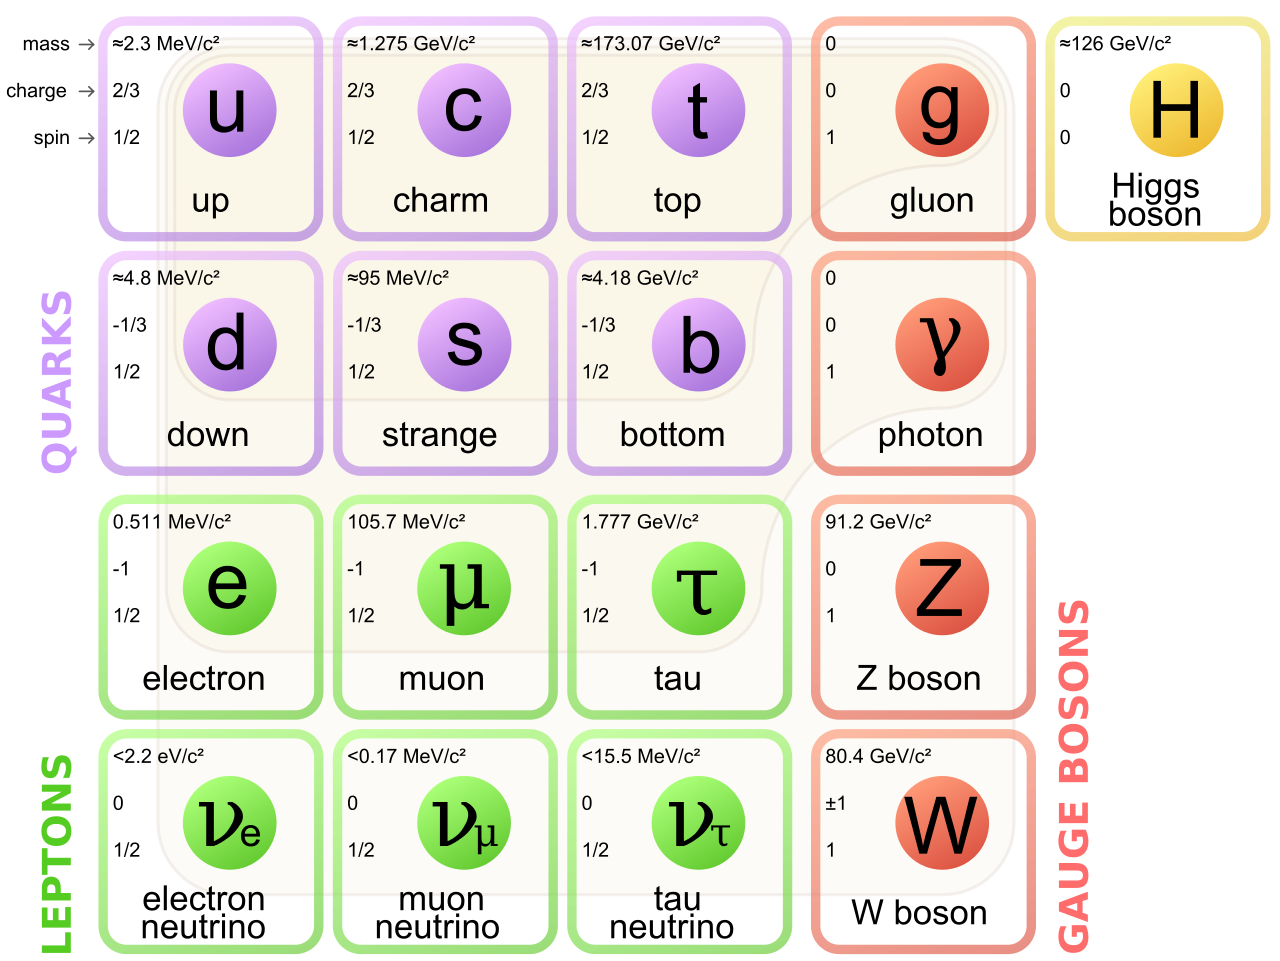
\includegraphics[width=\textwidth]{smparticles.png}
\end{figure}
\end{columns}
\end{frame}

\begin{frame}[label=sm2]
\frametitle{The Standard Model}
\begin{columns}
\column{.5\textwidth}
\begin{figure}
\centering
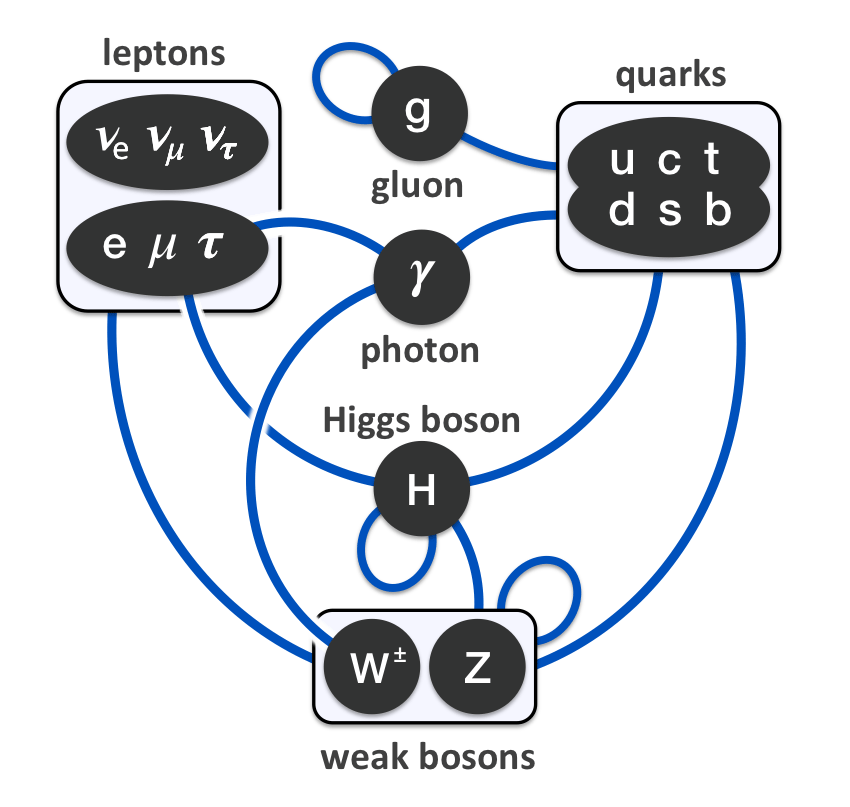
\includegraphics[width=\textwidth]{sminteractions.png}
\end{figure}
\column{.5\textwidth}
\begin{itemize}
    \item Interactions governed by SU(3)$_{C} \times$SU(2)$_L
        \times$U(1)$_Y$ gauge symmetry group
    \item Gluons, weak bosons, and the photon are the physical gauge
        bosons.
    \item The weak bosons acquire mass through
        \hlink{ewsb}{Electroweak Symmetry Breaking}
        (EWSB)
        brought on by the Higgs Mechanism.
\end{itemize}
\end{columns}
\end{frame}

\begin{frame}[t, label=proton_collision]
    \frametitle{Proton Collisions}
    \begin{columns}
        \column{.5\textwidth}
        \begin{itemize}
        \item Protons are
            \hlink{pdfs}{composite}
        \item Blue: collision
        \item Red: ``hard scatter''
        \item Purple: ``underlying event''
        \item Green: hadronization
        \item Gold: stable EM particles
        \end{itemize}
\column{.5\textwidth}
\begin{figure}
\centering
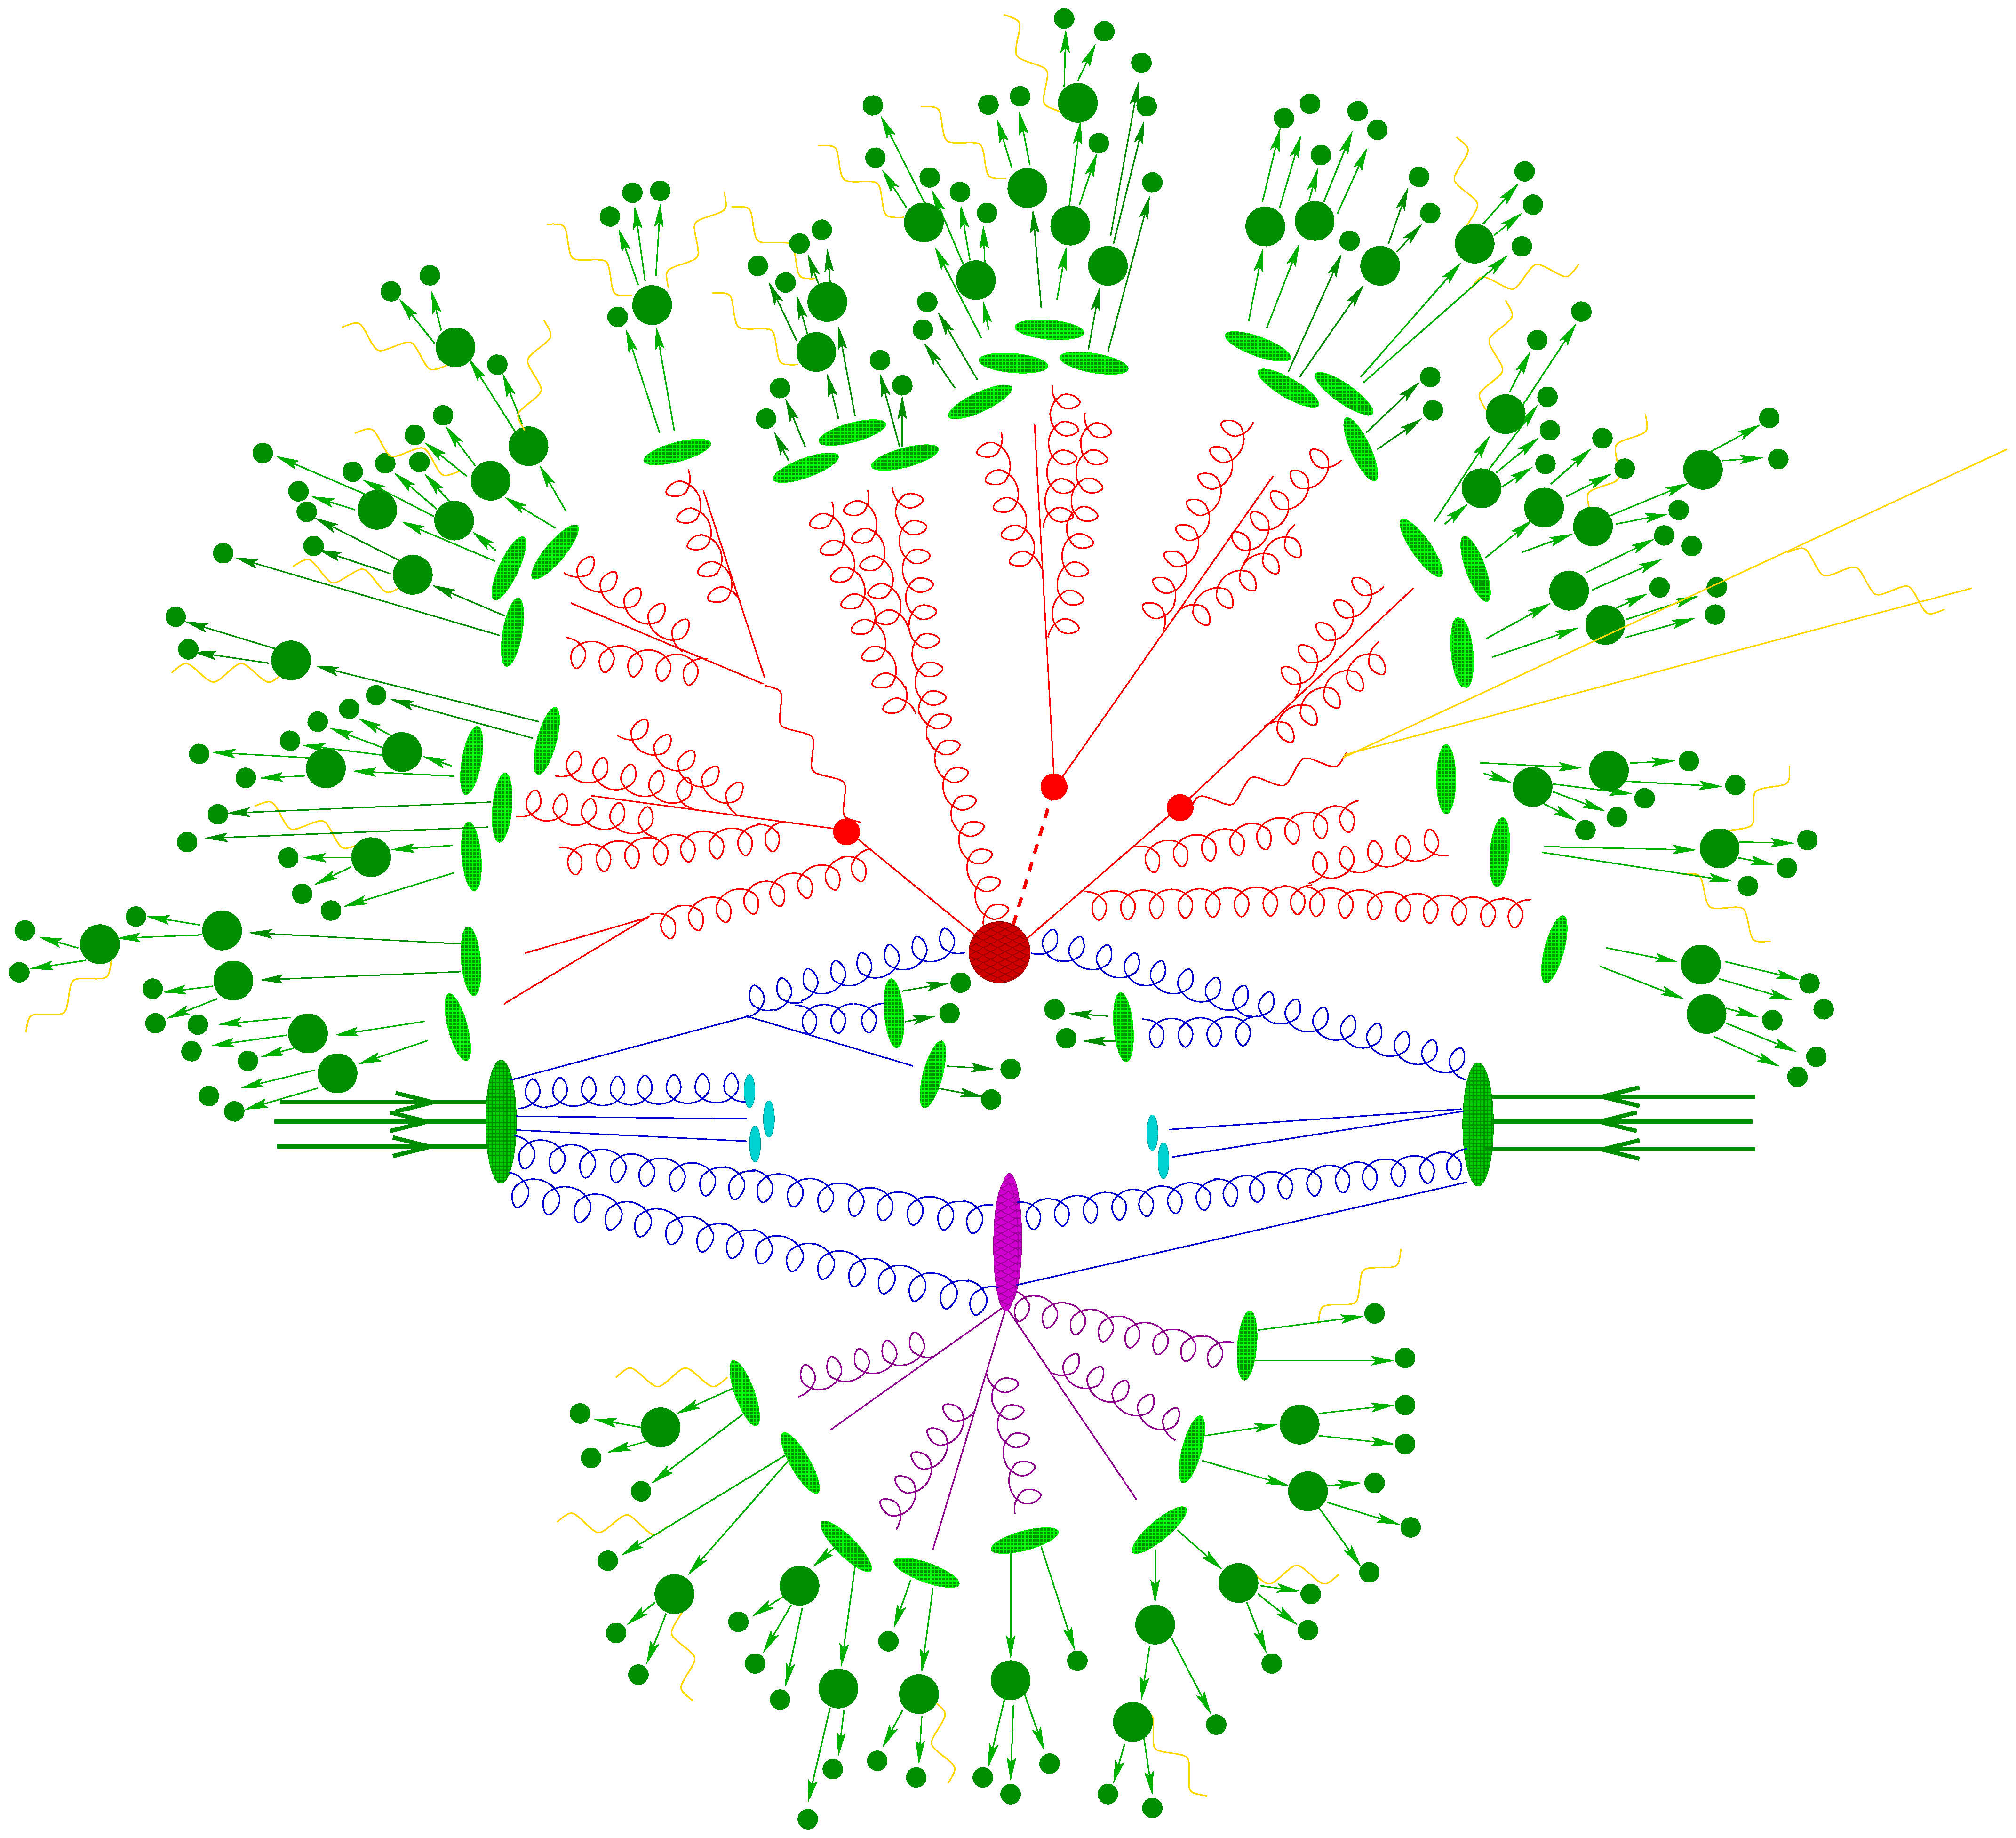
\includegraphics[width=\textwidth]{collision.eps}
\end{figure}
\end{columns}
\end{frame}

\subsection{Beyond the Standard Model Searches}

\begin{frame}
    \frametitle[label=bsm]{Beyond the Standard Model}
\begin{itemize}
    \item Despite its successes, the Standard Model is known to be an
        incomplete theory.
\begin{itemize}
    \item Gravitational force
    \item Dark matter and energy
    \item Asymmetry between matter and antimatter
    \item Disparity in fermion masses
    \item Gravitational and electroweak energy scales
    \end{itemize}
    \item New models address these issues, but they need to be tested
        experimentally!
\end{itemize}
\end{frame}

\begin{frame}
    \frametitle{Why \hlink{topprops}{Top Quarks}?}
\begin{columns}
\column{.5\textwidth}
\begin{itemize}
    \item Masses of quarks and charged leptons determined by
        couplings to the Higgs boson: $m_f = y_f \frac{v}{\sqrt 2}$
    \item Only the top quark's coupling is $\mathcal{O}(1)$: suggests
        a special role beyond the SM\@.
    \item High-mass exotic particles with mass-dependent couplings to
        fermions will {\bf preferentially decay to top quarks}.
\end{itemize}
\column{.5\textwidth}
\begin{figure}
\centering
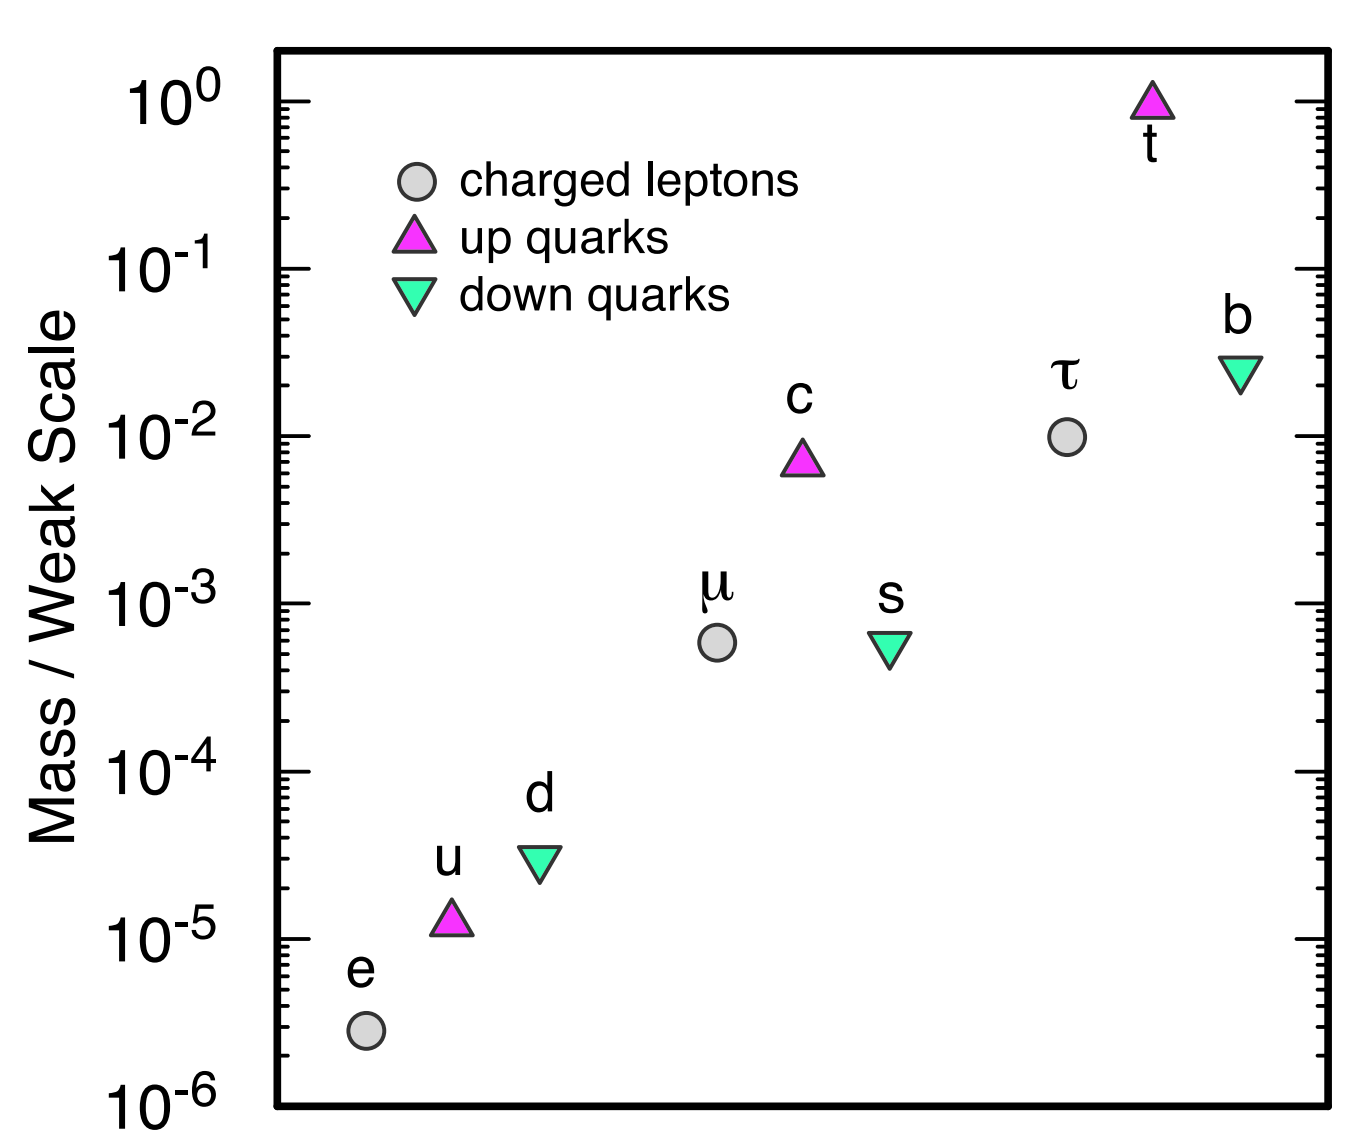
\includegraphics[width=\textwidth]{fermmass.png} % \cite{bib:fermmass}
\end{figure}
\end{columns}
\end{frame}

\begin{frame}
    \frametitle{\ttbar\ Resonances}
\centering
\begin{figure}
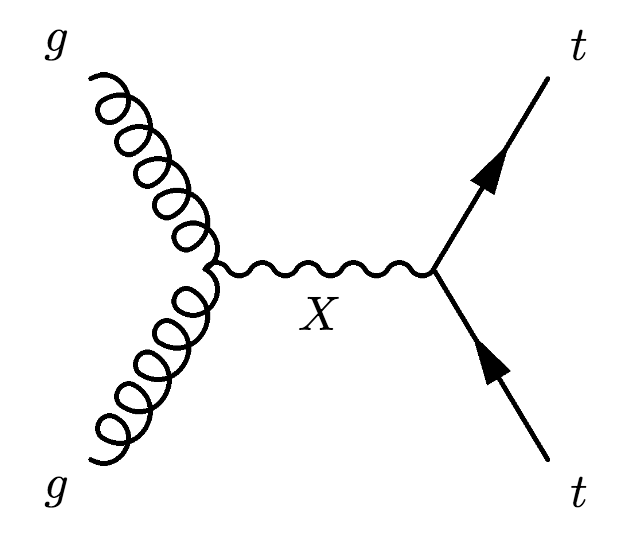
\includegraphics[width=.5\textwidth]{feynkkg.png}
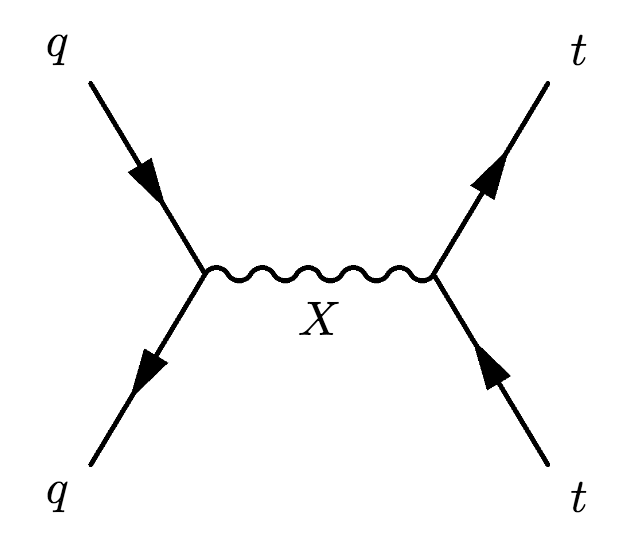
\includegraphics[width=.5\textwidth]{feynzp.png}
\end{figure}
\begin{itemize}
\item Exotic particles which couple to gluons or quarks can be created
    with a hadron collider.
\item If exotic particles are produced, a peak in the \mtt\ spectrum
    will result.
\end{itemize}
\end{frame}

\begin{frame}
\frametitle{Top Quark Pair Decay Channels}
\begin{columns}
\column{.5\textwidth}
\begin{itemize}
    \item Top quarks decay to a $b$ quark and a $W$ boson with
        probability $> 99.9$\%.
    \item The top pair decay channel is
        determined by the two $W$ boson decay modes.
    \item The $W$ boson branching fraction to each lepton flavor is
        10.5\%.
    \item 43.8\% of \ttbar\ pairs result in exactly one final state lepton.
\end{itemize}

\column{.5\textwidth}
\begin{figure}
\centering
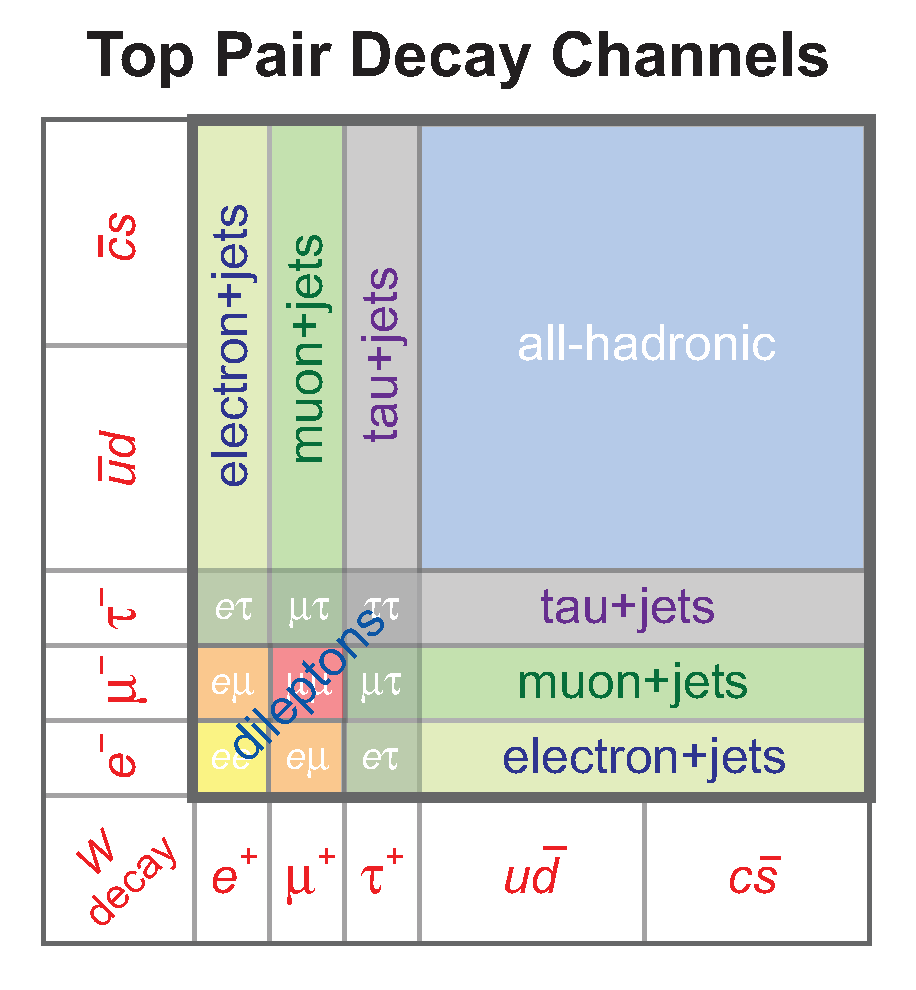
\includegraphics[width=\textwidth]{ttbardecaychannels.pdf}
\end{figure}
\end{columns}
\end{frame}

\subsection{Standard Model Backgrounds}

\begin{frame}
    \frametitle{Standard Model Background Processes}
    \centering
\begin{tabular}{l|r}
    \hline
    Process                         & Cross Section (pb) \\
    \hline
    Multijet                        & $72 \times 10^9$  \\
    \wjets\ ($W \to \ell \nu_\ell$) & $34 \times 10^3$  \\
    \zjets\ ($Z \to \ell\ell$)      & $2.9 \times 10^3$ \\
    \ttbar\ ($>= 1\ell$)            & 110               \\
    Single top ($>= 1\ell$)         & 49                \\
    $WW,WZ,ZZ$ ($>= 1\ell$)         & 17                \\
    \hline
    \hline
\end{tabular}

\vspace{1cm}

The important Standard Model backgrounds to possible resonant \ttbar\
production and their cross sections

\end{frame}

\begin{frame}
    \frametitle{SM Top Quark Pair Production}

\begin{figure}
\centering
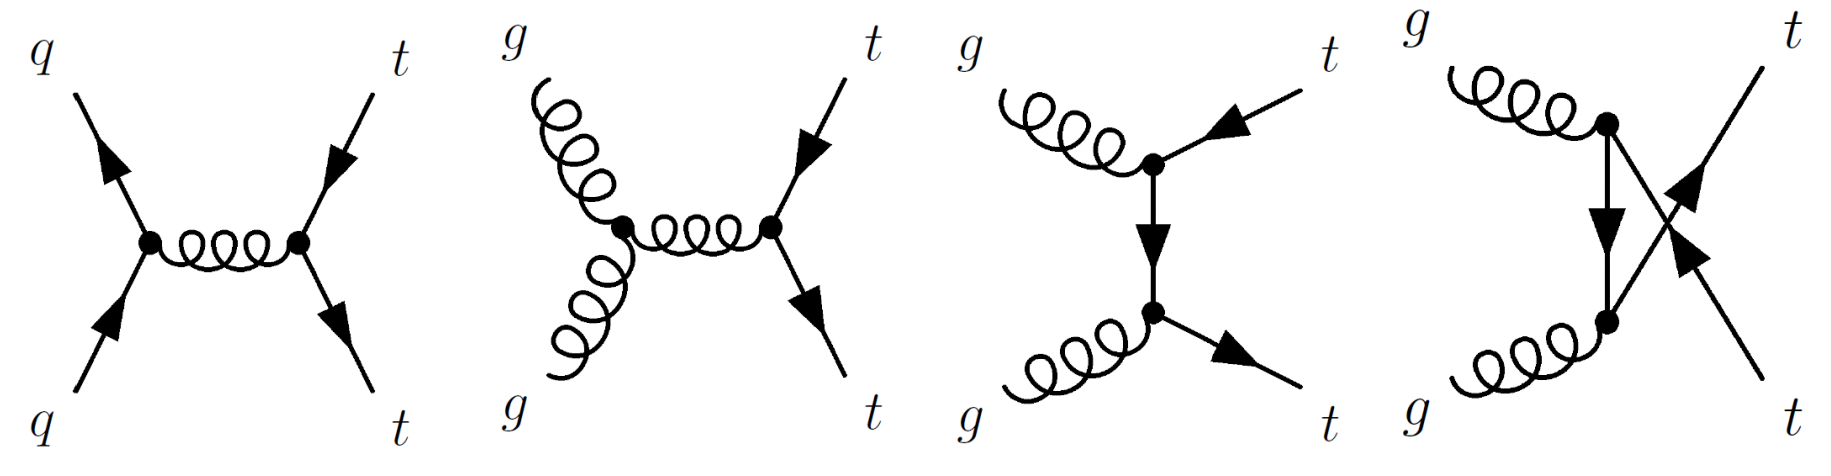
\includegraphics[width=\textwidth]{ttbardiagrams.png}
\end{figure}

\vfill

\begin{itemize}
    \item Top quarks are primarily produced at the Large Hadron
        Collider (LHC) through two SM processes:
    \begin{itemize}
            \item Quark-antiquark annihilation
            \item Gluon-gluon fusion
    \end{itemize}

    \item SM production of \ttbar\ pairs is {\bf not resonant}: if
        exotic particles are produced, a peak in the \mtt\ spectrum
        above the SM background will result.
\end{itemize}

\end{frame}
